\section{Техническое задание}
\subsection{Основание для разработки}

Основанием для разработки программного продукта служит задание по курсовой работе по дисциплине  "<Разработка web-форума \textquotedbl 8chan\textquotedbl\ на языке Python">.

\subsection{Цель и назначение разработки}

Основной задачей выпускной квалификационной работы является разработка web-форума.

Задачами данной разработки являются:
\begin{itemize}
\item создание разделов сайта с постами, профилём, постом непосредственно и главной страницы;
\item реализация формы для добавления постов и комментариев;
\item реализация формы для регистрации и авторизации;
\end{itemize}

\subsection{Требования пользователя к интерфейсу web-сайта}

Сайт должен включать в себя:
\begin{itemize}
    \item навигацию по темам;
    \item авторизацию и регистрацию;
    \item доступ для пользователя;
\end{itemize}

Композиция шаблона сайта представлена на рисунке ~\ref{templ:image}.

\begin{figure}[ht]
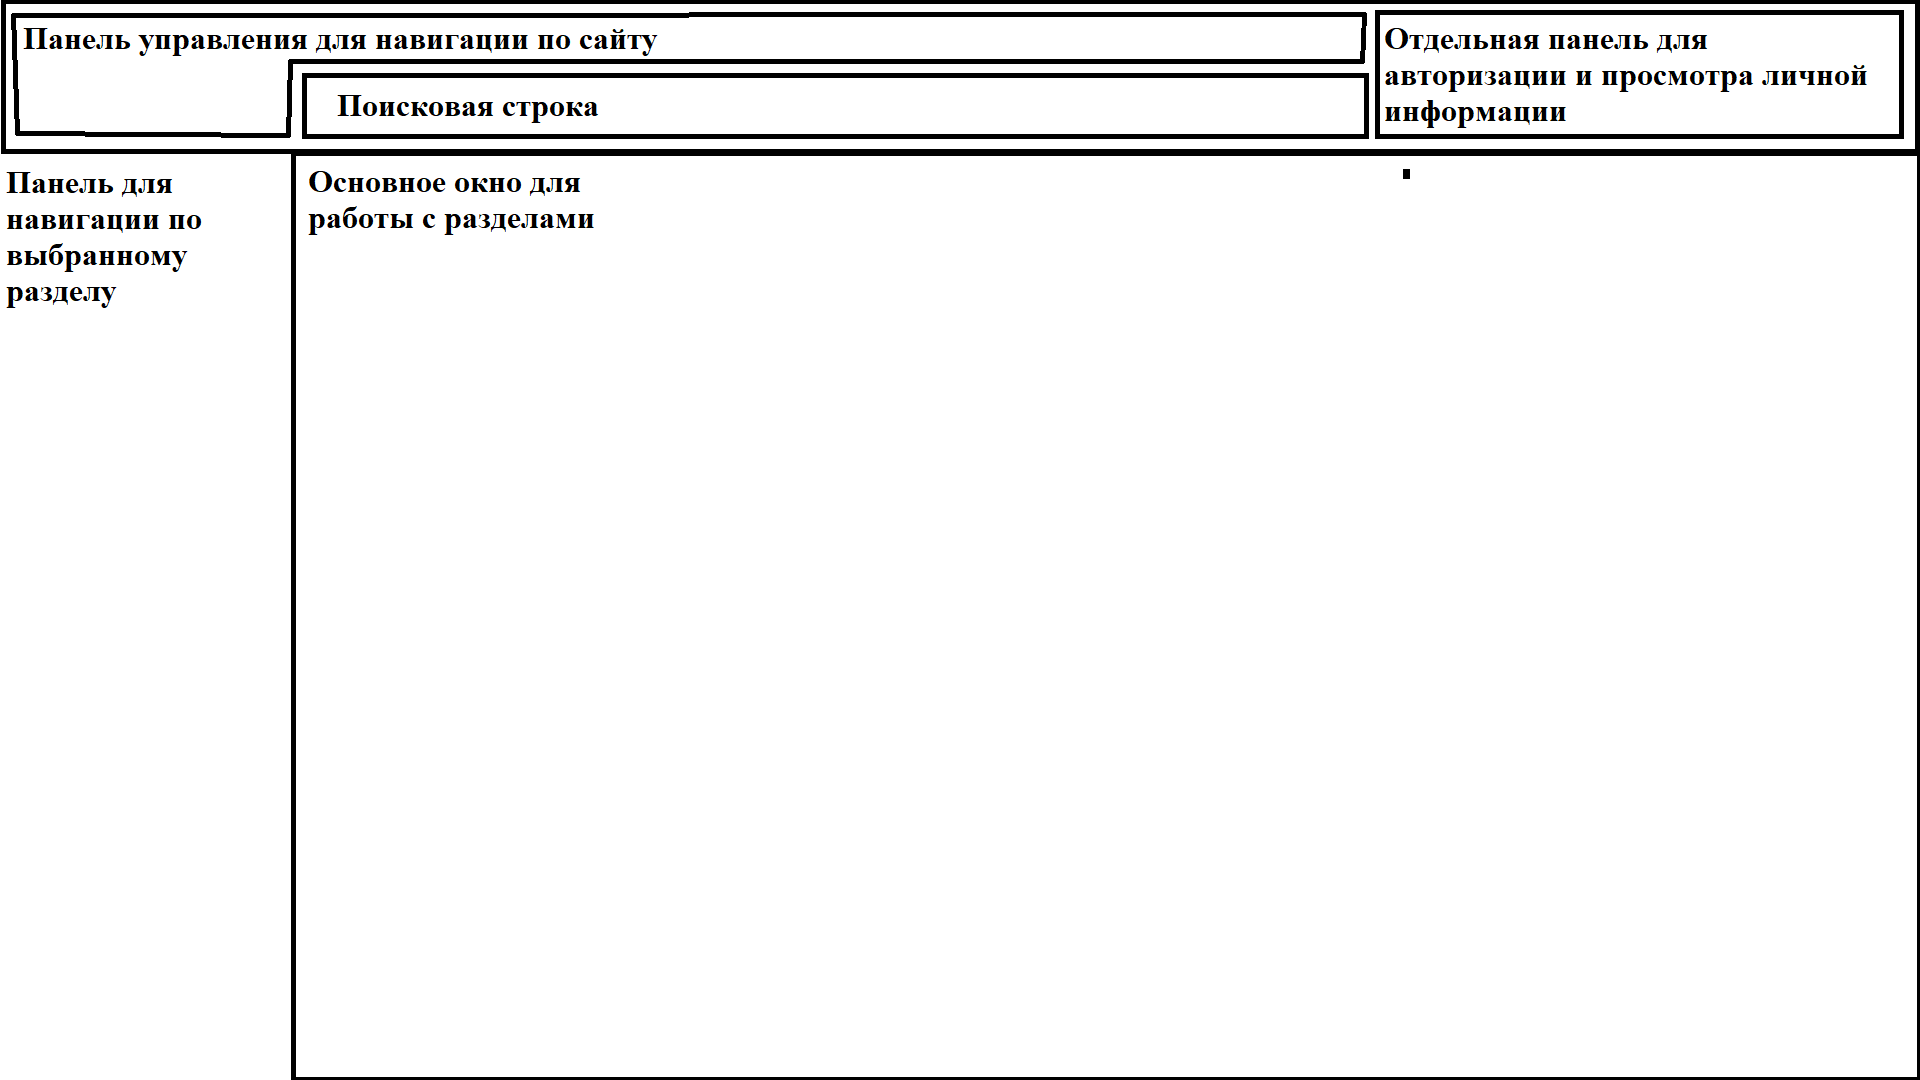
\includegraphics[width=1\linewidth]{templ}
\caption{Композиция шаблона сайта}
\label{templ:image}
\end{figure}
%\vspace{-\figureaboveskip} % двойной отступ не нужен (можно использовать, если раздел заканчивается картинкой)

\subsection{Моделирование вариантов использования}

Для разрабатываемого веб-сайта была создана модель, предоставляющая наглядное представление сценариев использования сайта. Эта модель является важным инструментом для физической разработки и подробного анализа взаимосвязей между объектами. При построении диаграммы вариантов использования используется унифицированный язык визуального моделирования (UML).

Диаграмма вариантов использования описывает функциональное предназначение разрабатываемой системы, представляя ее в виде ряда сценариев, предоставляемых системой актерам или сущностям, взаимодействующим с ней. Актерами являются внешние сущности, такие как пользователи или технические устройства, взаимодействующие с системой. Прецеденты описывают набор действий, предоставляемых системой актерам.

Таким образом, диаграмма вариантов использования служит начальным концептуальным представлением системы в процессе ее проектирования, представляя сценарии взаимодействия и действий, доступных пользователям и другим актерам.

На основании анализа предметной области в программе должны быть реализованы следующие прецеденты:
\begin{enumerate}
\item Регистрация нового пользователя
\item Авторизация пользователя
\item Добавление новой темы
\item Комментирование темы
\end{enumerate}

Диаграмма вариантов использования сайта представлена на рисунке 
~\ref{прецеденты:image}.

\begin{figure}[H]
	
	\center{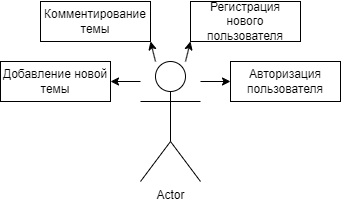
\includegraphics[width=0.7\linewidth]{прецеденты}}
	\caption{Прецеденты}
	\label{прецеденты:image}
\end{figure}

\subsubsection{Сценарии прецедентов программы}

\begin{enumerate}
	\item Сценарий для прецедента «Регистрация нового пользователя»:
	\begin{itemize}
		\item основной исполнитель: пользователь;
		\item заинтересованные лица и их требования: пользователю необходимо предоставить уникальный логин и пароль;
		\item предусловие: пользователь открыл веб-форум в браузере;
		\item основной успешный сценарий: пользователь вводит уникальный логин и пароль, система регистрирует нового пользователя.
	\end{itemize}
	\item Сценарий для прецедента «Авторизация пользователя»:
	\begin{itemize}
		\item основной исполнитель: пользователь;
		\item заинтересованные лица и их требования: пользователю необходимо предоставить зарегистрированный логин и пароль;
		\item предусловие: пользователь открыл веб-форум в браузере;
		\item основной успешный сценарий: пользователь вводит зарегистрированный логин и пароль, система производит авторизацию.
	\end{itemize}
	
	\item Сценарий для прецедента «Добавление новой темы»:
	\begin{itemize}
		\item основной исполнитель: пользователь;
		\item заинтересованные лица и их требования: пользователю необходимо написать заголовок темы и описание темы;
		\item предусловие: пользователь авторизован в системе;
		\item основной успешный сценарий: пользователь вводит заголовок темы и описание темы, добавляет её.
	\end{itemize}
	
	\item Сценарий для прецедента «Комментирование темы»:
	\begin{itemize}
		\item основной исполнитель: пользователь;
		\item заинтересованные лица и их требования: пользователю необходимо написать текст сообщения;
		\item предусловие: пользователь авторизован в системе;
		\item основной успешный сценарий: пользователь пишет текст сообщения, и отправляет его.
	\end{itemize}
	
\end{enumerate}

\subsection{Требования к оформлению документации}

Разработка программной документации и программного изделия должна производиться согласно ГОСТ 19.102-77 и ГОСТ 34.601-90. Единая система программной документации.
